\documentclass[a4paper,12pt]{article}

\usepackage{times}
\usepackage{changepage}
\usepackage{setspace}
\usepackage{caption}
\usepackage{sidecap}
\usepackage{graphicx}
\usepackage[document]{ragged2e}
\usepackage{amsmath}
\usepackage{import}
\DeclareMathSizes{12}{10}{10}{6}
\usepackage{geometry}
 \geometry{
 top=35mm,
 }

\begin{document}
\pagenumbering{gobble}
\setlength{\parindent}{0em}
\doublespacing
\captionsetup{labelformat=empty}

\begin{center}
{\huge PACCMAN User/Developer Guide}

(Python Analysis of Conformal Cooling Molds And/or desigNs)
\end{center}

\bigskip

This guide is meant to be used as a resource for using, adding to, or integrating the PACCMAN program. 
It is expected that users will have a package manager such as Anaconda or another program with Numpy, Scipy, Matplotlib, etc.

\medskip

In order to install Pytest with Anaconda, open the Anaconda Powershell Prompt and run the command "conda install -c anaconda pytest ".

\medskip

Feedback is welcome. Please report all bugs to hughfeehan353 on Github. Thanks.

\section*{Basic Use:}

When run, the program first presents three options.
\begin{adjustwidth}{1cm}{}
Selecting "N" uses the first mold material properties (KM1, etc.) and then asks the user to choose the heat transfer coefficient correlation.

Selecting "M" compares the three mold materials using the Gnielinski correlation.

Selecting "H" compares the three heat transfer coefficient correlations using the first mold material property (KM1, etc.).
\end{adjustwidth}

\medskip

For all three choices, the program asks the user if they would like to save graphs of the average heat cycle temperature over time.
\begin{adjustwidth}{1cm}{}
Choosing "Y", downloads the graph in .png and .eps formats.

Choosing "N" will not download the graphs
\end{adjustwidth}
\clearpage

\medskip
\begin{center}
\begin{figure}
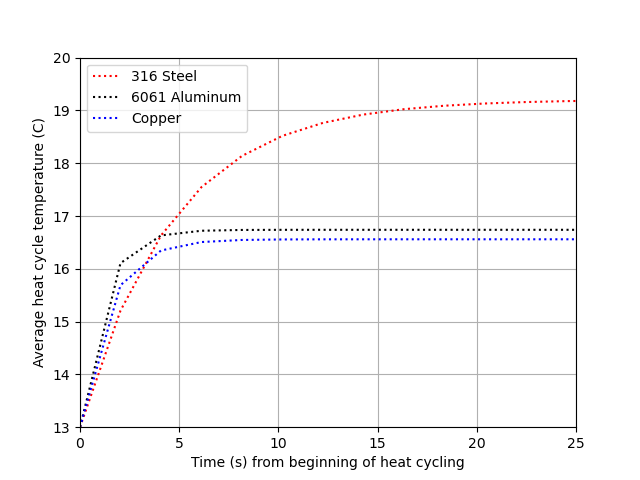
\includegraphics[width=\linewidth]{paccman-example-graph.png}
\caption{An example graph for option "M" (mold material comparison). }
\end{figure}
\end{center}

The program is written so that by changing the variables, it can analyize any desired conformal cooling design and will report the following data: 
\begin{adjustwidth}{1cm}{}

flow velocity, kinematic viscosity, Reynolds number, Prandl number, Darcy friction factor, heat transfer coefficient, average heat cycle temperature of the mold, time constant, and coolant pressure drop.

\end{adjustwidth}
\clearpage

\section*{Multiple Variables / Arrays}

Arrays can be used in this program to compare either multiple values for a single variable or multiple values for multiple values.

\medskip

When comparing multiple values for a single variable, use a NumPy array and the program will compare the efficacy of the values entered.

\medskip 

When inputting multiple values for multiple variables, the number of values in each array must be the same. The values in array position 1 will always do arithmetic from the other values in position 1, the values in position 2 work with the other values in position 2, etc.. The final results that the program give will be the same as the number of array variables, which must be the same for every array. A recommended use of this is  comparing different materials for the mold, coolant, or part and putting all the material properties of the same material in the same array slot.

\clearpage

\section*{Application Fundamentals for Advanced Use:}

At the beginning, the program initializes and assigns all the basic variables. By default, these are imported from the "basedata.py" file. 

\medskip

In order to change the values, the data in this file can either be edited directly or the import location can be changed. In order to do this, locate the import statement on line 12 of "paccman.py" and change "basedata" to the desired new file. All of the variables in "basedata.py" are necessary for the program to function properly so none should not be completely omitted if a new file is used.

\medskip

Afterwards, all the necessary functions are defined. These cannot be removed as they are necessary for the program’s function but could be added to.

\medskip

At this point there is an “if” statement to check for the user’s desired function for the program.  This “if” statement contains all of the program’s calculation functions in order to ensure that nothing will break if the user chooses an invalid letter.

\medskip

The first thing inside the “if” statement are some calculations that must be completed no matter the chosen choice of the program’s function. 

\medskip

The rest of the calculations contain nested “if” and “elif” statements so that the correct variables are used for the chosen program function.

\medskip

Once the calculations are completed, the program creates a plot of the average heat cycle temperature over time that the user has the choice of downloading.

\medskip

The program can be tested using Pytest by running the "pytest" command in the program's directory.

\clearpage

\section*{Variables Used:}

\medskip

Part Thickness: $L_{P}$

Coolant Line Diameter: $D$

Average Height of Coolant Line Surface Irregularties: $\varepsilon$

Coolant Line Length: $L$

Coolant Thermal Conductivity: $K_{C}$

Coolant Density: $\rho_{C}$

Mold Specific Heat Capacity: $C_{C}$

Coolant Temperature: $T_{C}$

Part Density: $\rho_{P}$

Part Specific Heat Capacity: $C_{P}$

Thermal Conductivity of Mold: $K_{M}$

Coolant Line Pitch Distance: $W$

Distance from Coolant Line to Mold Wall: $L_{M}$

Difference in Part Temperature Between Inserted Into Mold and Released: $T$

Cycle Time: $T_{Cycle}$

Mold Density: $\rho_{M}$

Mold Specific Heat Capacity: $C_{M}$

Initial Mold Temperature: $T_{MO}$

Coolant Flow Rate: $\dot{V}$

Coolant Dynamic Viscosity: $\mu$

Coolant Dynamic Viscosity When Near Wall: $\mu_{W}$

\clearpage

\section*{Equations Used:}

\medskip

Flow Velocity of Coolant (U): $\dfrac{\dot{V}}{\pi \cdot (\dfrac{D}{2})^{2}}$

\medskip

Coolant Kinematic Viscosity (KV): $\dfrac{\mu}{\rho_{C}}$

\medskip

Reynolds Number (Re): $\dfrac{U \cdot D}{KV}$

\medskip

Prandtl Number (Pr): $\dfrac{\mu \cdot C_{C}}{K_{C}}$

\medskip

Darcy Friction Factor (Haaland Equation) (f): $(\dfrac{1}{-1.8log[(\dfrac{\varepsilon}{3.7 \cdot D})^{1.11}+(\dfrac{6.9}{Re})]})^{2}$

\medskip

There are three chooseable equations for the Nusselt Number (Nu):

1. Dittus-Boelter: $0.023 \cdot Re^{\frac{4}{5}} \cdot Pr^{0.4}$

\medskip

2. Gnielinski: $\dfrac{\dfrac{f}{8} \cdot (Re-1000) \cdot Pr}{1 + [12.7 \cdot (\dfrac{f}{8})^{0.5} \cdot (Pr^{\frac{2}{3}}-1)]}$

\medskip

3. Sieder-Tate: $0.027 \cdot Re^{\frac{4}{5}} \cdot Pr^{\frac{1}{3}} \cdot (\frac{\mu}{\mu_{W}})^{0.14}$

\medskip

Heat Transfer Coefficient (h): $\dfrac{K_{C}}{D} \cdot Nu$

\medskip

Average Temperature of the Mold (ATM): $T_{C} + \dfrac{\rho_{P} \cdot C_{P} \cdot L_{P} \cdot T \cdot [(2 \cdot K_{M} \cdot W) + (h \cdot \pi \cdot D \cdot L_{M})]}{h \cdot \pi \cdot D \cdot K_{M} \cdot T_{Cycle}}$ 

\medskip

Time Constant ($T_{Constant}$): $\dfrac{\rho_{M} \cdot C_{M} \cdot L_{M}^{2}}{K_{M}} \cdot (1 + \dfrac{2 \cdot W \cdot K_{M}}{h \cdot \pi \cdot D \cdot L_{M}})$

\medskip

Pressure Drop: $\dfrac{Df \cdot L}{D} \cdot \dfrac{\rho_{C}}{2} \cdot \dot{V}^{2}$

\medskip

Equation for Graphs: $y = ATM + (T_{MO} - ATM) \cdot e^{\dfrac{-x}{T_{Constant}}}$

\clearpage

\section*{Test Cases:}

This folder contains two samples of data for use in the PACCMAN program.  The data contained by the "xucomparison" file contains values from the 2001 paper: The Design of Conformal Cooling Channels in Injection Molding Tooling" by Xiorong Xu, Emanuel Sachs, and Samuel Allen. "xucomparison.csv" is a table produced through WebPlotDigitizer of Figure 4 in the Xu paper. The data contained by the "guilongcomparison" file is from the 2010 paper "Analysis of thermal cycling efficiency and optimal design of heating/coolingsystems for rapid heat cycle injection molding process" by Wang Guilong, Zhao Guoqun, Li Huiping, and Guan Yanjin. "guilongcomparison.csv" contains the data from Figure 6 pulled with WebPlotDigitizer. There are also .png files graphically comparing the real world results of these papers to the program's created graphs.


\end{document}